\documentclass[
%% TIKZ_CLASSOPTION %%
tikz
]{standalone}
\usepackage{amsmath}
\usetikzlibrary{matrix}
%% EXTRA_TIKZ_PREAMBLE_CODE %%
\begin{document}
%% TIKZ_CODE %%
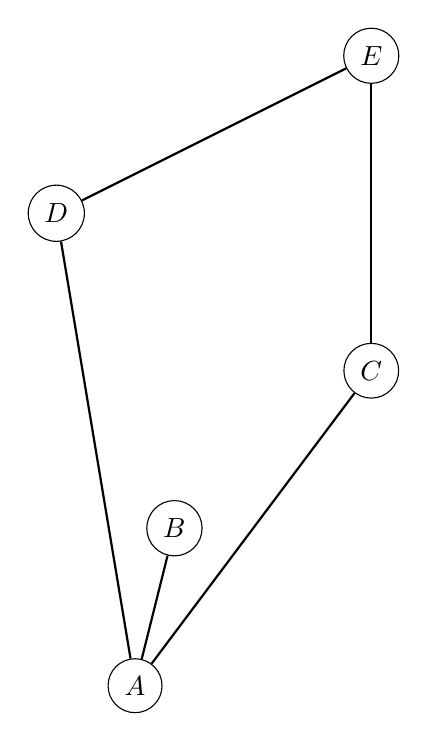
\begin{tikzpicture}

\tikzset{vertex/.style = {shape=circle,draw,minimum size=1.5em}}
\tikzset{edge/.style = {->,> = latex}}

\node[vertex] (a1) at (0,-1) {$A$};
\node[vertex] (b1) at (0.5,1) {$B$};
\node[vertex] (c1) at (3,3) {$C$};
\node[vertex] (d1) at (-1,5) {$D$};
\node[vertex] (e1) at (3,7) {$E$};

\draw[thick] (a1) -- (b1);
\draw[thick] (a1) -- (c1);
\draw[thick] (a1) -- (d1);
\draw[thick] (e1) -- (c1);
\draw[thick] (d1) -- (e1);

\end{tikzpicture}
\end{document}
